\documentclass[10pt, a4paper]{beamer}
\usepackage{graphicx}
\usetheme{Berkeley}
\usecolortheme{sidebartab}

\begin{document}
	\setbeamertemplate{sidebar left}{}
	\title{Progress Presentation-I}
	\subtitle{e-Yantra Summer Internship-2016 \\ Question Bank Management}
	\author{Bhalchandra Naik\\Tushar Shah\\
	\vspace{5mm}
	Mentors: Shubham Gupta\\Uttam Kumar Gupta\\Yogita Mali\\}
	\institute{IIT Bombay}
	\date{30th June,2016}
	%\addtobeamertemplate{sidebar left}{}{\includegraphics[scale = 0.3]{logowithtext.png}}
	\frame{\titlepage}

\setbeamertemplate{sidebar left}[sidebar theme]

%%%%%%%%Overview of the Project%%%%%%%%%
\section{Overview of Project}
\begin{frame}{Overview of Project}
	Give following details: \\
	\begin{itemize}
		\item Project Name: Question Bank Management	 \\
			
		\item Objective
			\begin{enumerate}
				\item To develop a web-based application that enables users to create questions and get them reviewed by peers over the application
				\item The question or any of its attributes might be edited by users with review rights which is why the application must implement version control over the questions.
			\end{enumerate}
		\item Deliverables
			\begin{enumerate}
				\item Question Bank Management System with all the specified features
				\item A comprehensive developer manual and user manual
			\end{enumerate}
	\end{itemize}
\end{frame}

%%%%%%%%%Features%%%%%%%%%%%
\section{Features}
\begin{frame}{Features}
	Give following details: 
	\begin{itemize}
	
		\item Creation of Questions	 
			\begin{enumerate}
				\item Questions must have attributes like difficulty level, time required etc
				\item Equation box(\LaTeX  to image)
			 	\item Adding diagrams
				\item Each questions must have tags pertaining to its subject matter
            \end{enumerate}			
            
            			
		\item Revision Histiory of Questions
			\begin{enumerate}
				\item Each question is reviewed by several peers of the creator, chosen selectively or randomly by the admin
				\item The application must maintain records of each version of the questions post every review
			\end{enumerate}
			
	\end{itemize}
\end{frame}

%%%%%%%%%%Overview of Task%%%%%%%%%%%
\section{Overview of Task}
\begin{frame}{Overview of Task}

	\begin{tabular}{|p{7mm}|p{5cm}|c|}
		
		\hline
		\textbf{Sr. no.} & \textbf{Task} & \textbf{Deadline} \\
		
		\hline
		\scriptsize{1}&\scriptsize{The SRS (Software Requirements Specification)} & \scriptsize{3 Days}\\
		
		\hline
		\scriptsize{2}&\scriptsize{Set up and study Laravel and Database Management} & \scriptsize{4 Days}\\
		
		\hline
		\scriptsize{3}&\scriptsize{Schema Development (Rough draft)} & \scriptsize{1 Days}\\
		
		\hline
		\scriptsize{4}&\scriptsize{Basic GUI development} & \scriptsize{3 Days}\\	
		
		\hline
		\scriptsize{5}&\scriptsize{Account management (including access management) } & \scriptsize{3 Days}\\
		
		\hline
		\scriptsize{6}&\scriptsize{Adding   features   like   adding/editing/reviewing   question,   tag suggestion,   adding   equations,   diagrams,   text   to   image   conversion  
etc.  } & \scriptsize{8 Days}\\

		\hline
		\scriptsize{7}&\scriptsize{Testing and Debugging} & \scriptsize{4 Days}\\
		
		\hline		
		\scriptsize{8}&\scriptsize{Documentation} & \scriptsize{4 Days}\\	
		\hline	
	\end{tabular} 
\end{frame}

\section{Task Accomplised}
\begin{frame}{Task Accomplised}
	\begin{itemize}
		\item Software Requirements Specification is finalised
		\item Basic GUI
		\item Creation of users by admin
		\item Detailed UI for creating a question is ready(converting \LaTeX code to image, selecting tags, addition of Math Symbols to Question description,text to image conversion.
		\item Account management
	\end{itemize}
\end{frame}

\section{Snapshots}
\begin{frame}{Snapshots}
	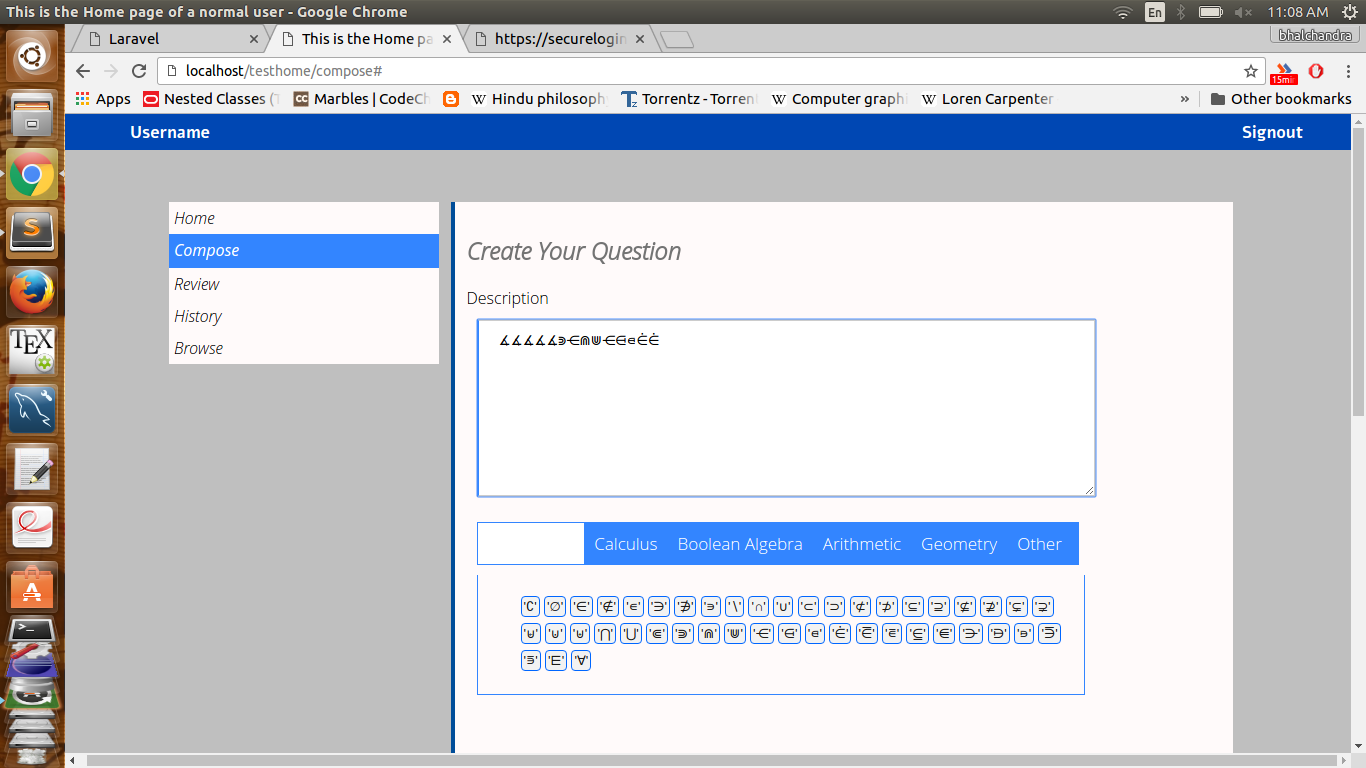
\includegraphics[scale=0.08]{photo1.png}\hspace{1cm}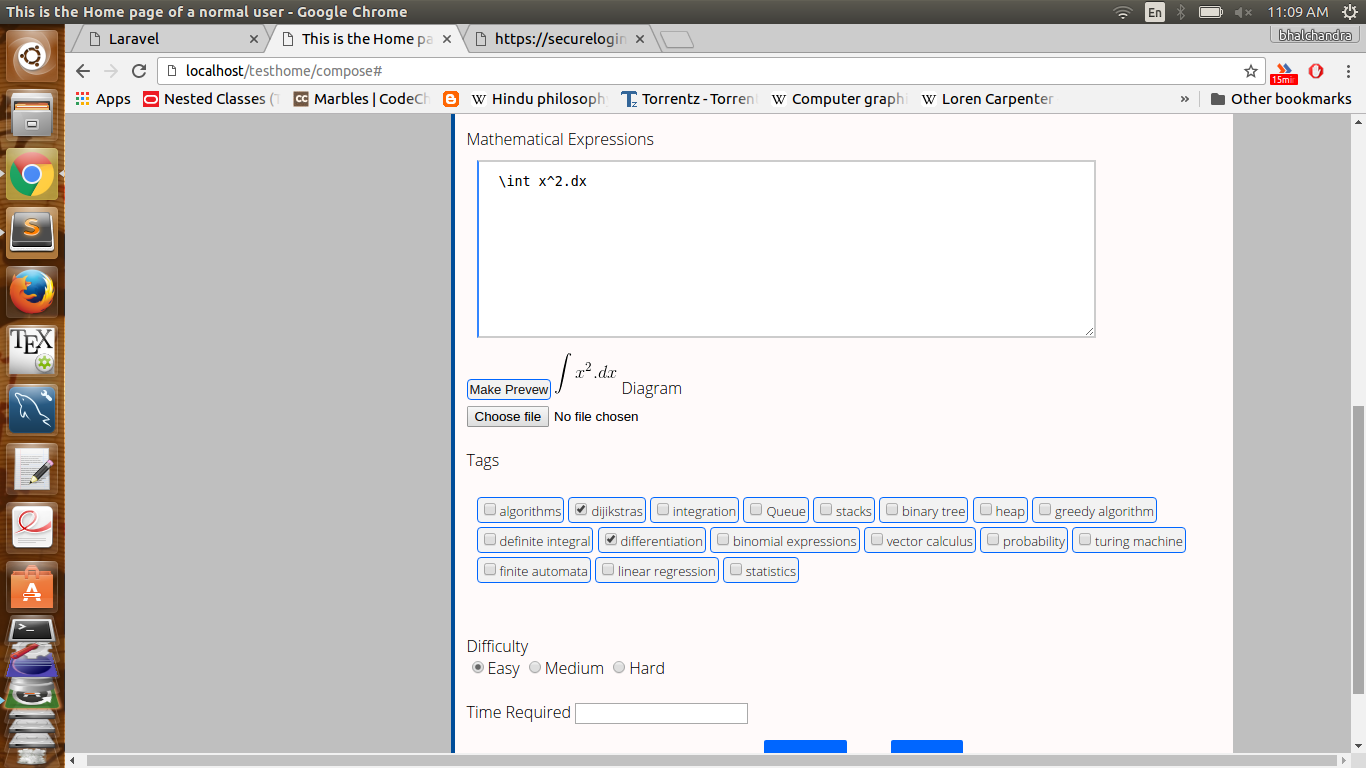
\includegraphics[scale=0.08]{photo2.png}\\
	\vspace{2mm} 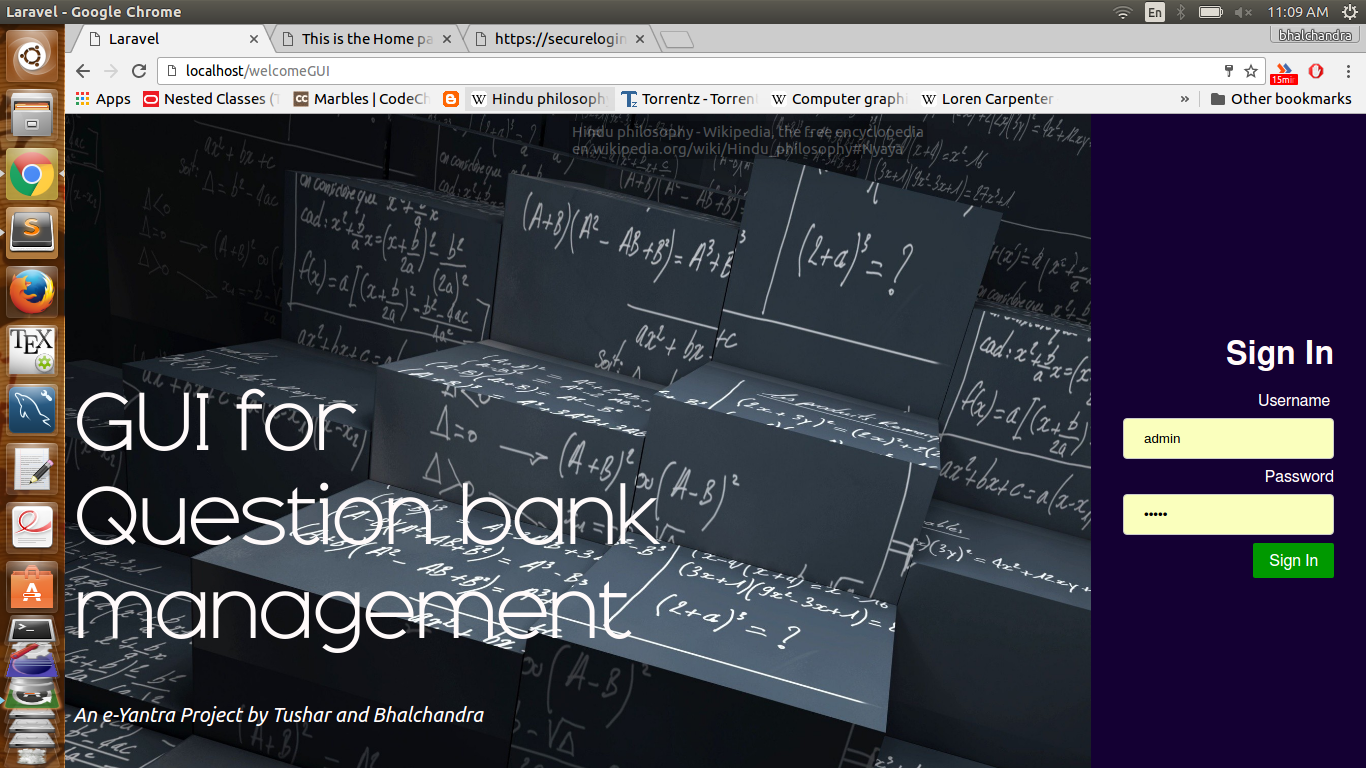
\includegraphics[scale=0.08]{photo3.png} \hspace{1cm}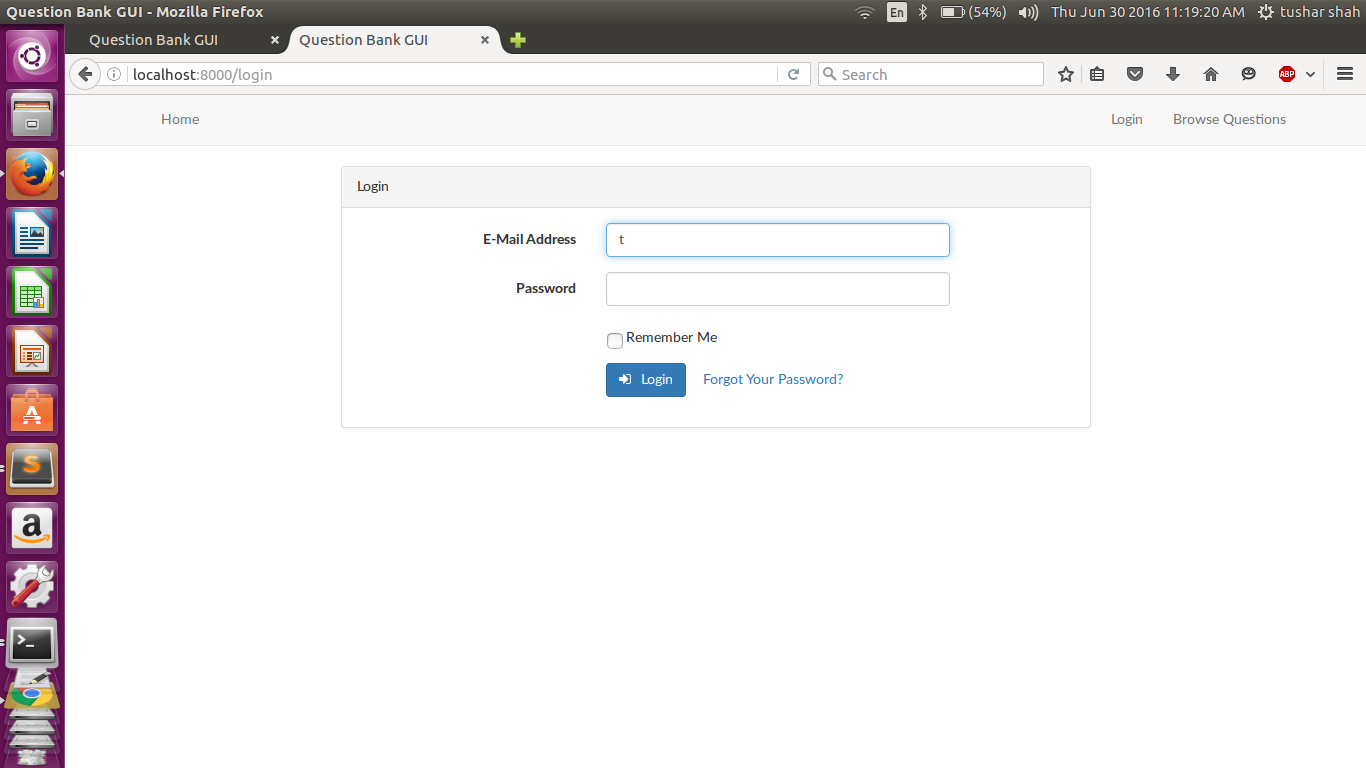
\includegraphics[scale=0.08]{photo4.png}\\
	\vspace{2mm} 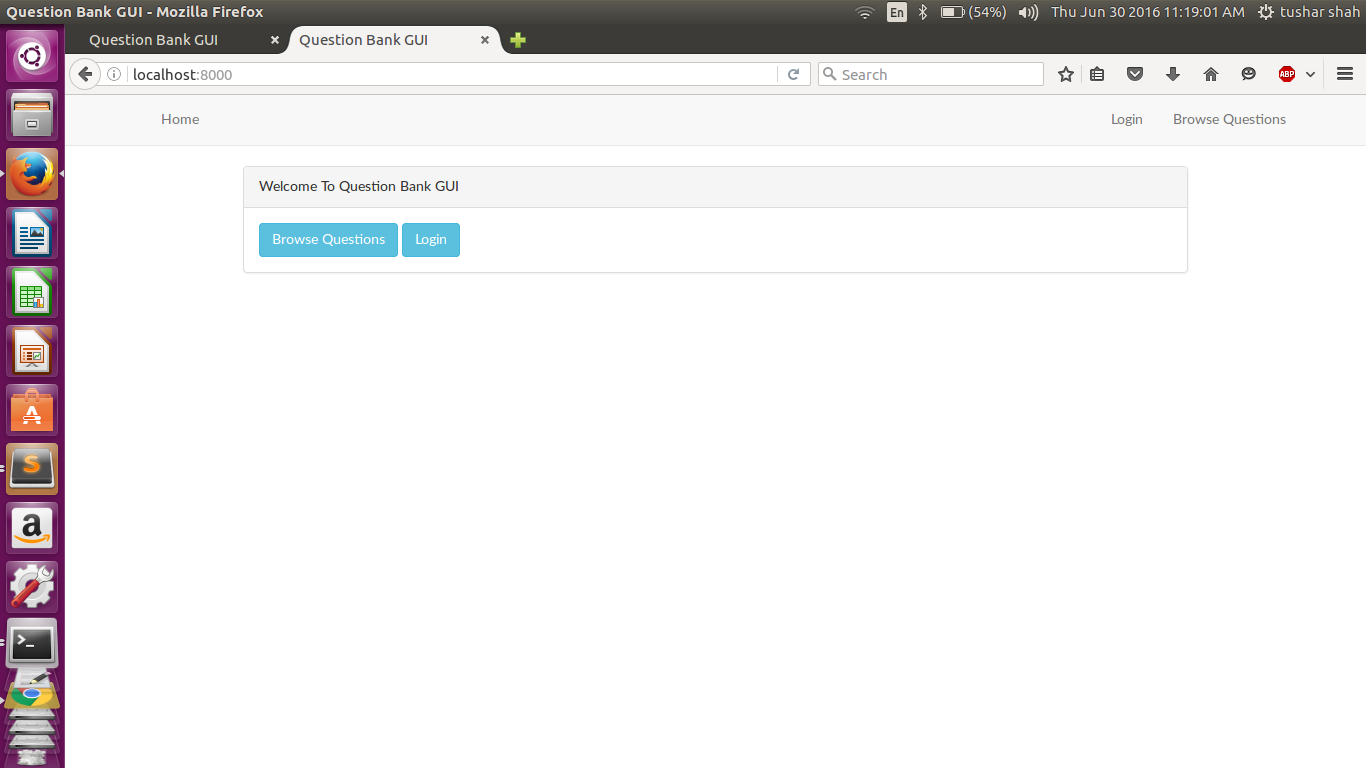
\includegraphics[scale=0.08]{photo5.png} 
\end{frame}

\section{Challenges Faced}
\begin{frame}{Challenges Faced}
	\begin{itemize}
		\item Learning Laravel
		\item Password Reset Link
		\item Finding APIs for some features of Question creation
	\end{itemize}
\end{frame}

\section{Future Plans}
\begin{frame}{Future Plans}
	\begin{itemize}
		\item Adding features like editing and reviewing
		\item Storing questions in the backend for Question Creation
		\item Browsing the Question Bank 
	\end{itemize}
\end{frame}


\section{Thank You}
\begin{frame}{Thank You}
	\centering \textit{\LARGE{Thank You!}}
\end{frame}
\end{document}
\grid
